\documentclass[11pt]{article}

% Packages
\usepackage{fullpage,amsthm,amsmath,amsfonts,graphicx,tikz,color,enumerate,algorithmic,hyperref,bbm,xifthen}
%\usepackage[numbered,framed]{mcode}
%\usepackage{framed}
\usepackage[section]{algorithm}

% For graphs and pictures
\usepackage{tkz-euclide}
\usetkzobj{all}
\usepackage{pgfplots}
\pgfplotsset{compat=1.11}
\tikzset{
	every pin/.style={fill=yellow!50!white,rectangle,rounded corners=3pt},
	small dot/.style={fill=black,circle,inner sep=1pt}
}

% Algorithm package
\renewcommand{\algorithmicrequire}{\textbf{Input:}}
\renewcommand{\algorithmicensure}{\textbf{Output:}}
\renewcommand{\algorithmiccomment}[1]{/* #1 */}
%\renewcommand\theContinuedFloat{.\alph{ContinuedFloat}}

% No Indent
\setlength\parindent{0pt}

% Theorem Style
\theoremstyle{definition}
\newtheorem{prop}{Proposition}[section]
\newtheorem{lemma}[prop]{Lemma}
\newtheorem{conjecture}[prop]{Conjecture}
\newtheorem{thm}[prop]{Theorem}
\newtheorem{hyp}[prop]{Hypothesis}
\newtheorem{cor}[prop]{Corollary}
\newtheorem{claim}[prop]{Claim}
\newtheorem{rmk}[prop]{Remark}
\newtheorem{notation}[prop]{Notation}
\newtheorem{defn}[prop]{Definition}
\newtheorem{eg}[prop]{Example}


% New Commands
\newcommand{\brac}[1]{\left(#1\right)}
\newcommand{\sqbrac}[1]{\left[#1\right]}
\newcommand{\curlbrac}[1]{\left\{#1\right\}}
\newcommand{\pbrac}[1]{\left\langle#1\right\rangle}

\newcommand{\diff}[2]{\frac{d\ifthenelse{\equal{#1}{}}{}{#1}}{d#2}}
\newcommand{\pardiff}[2]{\frac{\partial #1}{\partial #2}}

\newcommand{\abs}[1]{\left\lvert#1\right\rvert}
\newcommand{\norm}[1]{\left\lVert#1\right\rVert}
\newcommand{\normHTwo}[1]{\left\lVert#1\right\rVert_{H^2}}

\newcommand{\ceil}[1]{\left\lceil#1\right\rceil}
\newcommand{\floor}[1]{\left\lfloor#1\right\rfloor}

\newcommand{\E}[1]{\mathbb{E}\left[#1\right]}
\newcommand{\V}[1]{\mathbb{V}\left[#1\right]}
\newcommand{\F}[1]{\mathcal{F}_{#1}}
\newcommand{\N}{\mathbb{N}}
\newcommand{\R}{\mathbb{R}}
\newcommand{\C}{\mathbb{C}}
\newcommand{\Q}{\mathbb{Q}}
\newcommand{\Z}{\mathbb{Z}}
\newcommand{\W}{\mathbb{W}}
\newcommand{\prob}[1]{\mathbb{P}\left[#1\right]}
\newcommand{\ind}[1]{\mathbbm{1}_{\left\{#1\right\}}}
\newcommand{\real}[1]{\mathbb{R}^{#1}}
\newcommand{\hTwo}{H^2}
\newcommand{\vmin}[2]{#1 \wedge #2}

\newcommand{\repart}[1]{\text{Re}\brac{#1}}
\newcommand{\impart}[1]{\text{Im}\brac{#1}}

\newcommand{\normcdf}[1]{\text{N}\brac{#1}}
\newcommand{\normpdf}[1]{\text{N}'\brac{#1}}

\newcommand{\vega}{\nu}
\newcommand{\dt}{\delta t}
\newcommand{\dy}{\delta y}
\newcommand{\Zone}{Z^1_t}
\newcommand{\Ztwo}{Z^2_t}

% Colours
\newcommand{\red}[1]{{\color{red}#1}}
\newcommand{\cyan}[1]{{\color{cyan}#1}}
\newcommand{\yellow}[1]{{\color{yellow}#1}}
\newcommand{\green}[1]{{\color{green}#1}}
\newcommand{\orange}[1]{{\color{orange}#1}}

\begin{document}
\tableofcontents
\pagebreak
\section{Maths Basics}
\subsection{Functions}
	\begin{defn}
		A \emph{function} is a map from one set to another. We write $f:X\rightarrow Y$ which $f$ is the function which maps elements $x\in X$ to $y\in Y$. Another restriction we have is that for a given element $x\in X$, $f$ maps it to at most one element $y\in Y$.
	\end{defn}
	
	There are many different ways to write a function, let us consider the doubling function then we can write:
	\begin{eqnarray*}
		f(x) &=& x^2\\
		x &\mapsto & x^2\\
		f:x&\mapsto & x^2
	\end{eqnarray*}
	\begin{defn}
		Let $f:X\rightarrow Y$ be a function. Then $X$ is the \emph{domain} of $f$ and $Y$ is the \emph{image} of $f$.
	\end{defn}
	\begin{defn}
		Let $f:X\rightarrow Y$ be a function.
		\begin{enumerate}
		\item If $\forall x\in X, \exists ! y\in Y : f\brac{x} = y$ then $f$ is a \emph{one to one} mapping.
		\item If $\exists y\in Y, x_1, x_2 \in X : f\brac{x_1} = f{x_2} = y$ then $f$ is a \emph{many to one} mapping.
		\item Let $g: X \rightarrow Y$ be a mapping such that $\exists x\in X, y_1,y_2\in Y : f(x) = y_1 = y_2$ then $f$ is a \emph{one to many} mapping and it is not a function.
		\end{enumerate}
	\end{defn}
	\begin{defn}
		Let $f:X\rightarrow Y$ be a function. We say $f^{-1}$ is the \emph{inverse} map of $f$ if the following holds:
		$$ f^{-1}\brac{f\brac{x}} = f\brac{f^{-1}\brac{x}} = x, \quad \forall x\in X$$
	\end{defn}
	\begin{defn}
		Let $f: X\rightarrow Y$ be a function. 
		\begin{enumerate}
		\item We say $f$ is an \emph{even} function if $f\brac{-x} = f\brac{x},\forall x\in X$.
		\item We say $f$ is an \emph{odd} function if $f\brac{-x} = -f\brac{x},\forall x\in X$.
		\item Let $z\in X$, we say $f$ is \emph{periodic} with period $z$ if $ f\brac{x+z} = f\brac{x}, \forall x \in X$.
		\end{enumerate}
	\end{defn}
	\begin{defn}
		Let $f: X\rightarrow Y$ be a function.
		\begin{enumerate}
		\item We call $f$ an \emph{explicit} function if $forall y\in Y$ we can write $y = f\brac{x}$ for some $x\in X$ where all the terms of $x$ are on the right hand side of the equation. Sometimes, we will not be able to do that so that we have to write it as $f\brac{x,y} = 0$ which is called an \emph{implicit} function.
		\end{enumerate}
	\end{defn}
	The following is an example of an implicit function as we can write it with just $y$ on the left side of the equation with all the terms of $x$ on the right hand side:
	$$ 4y^4 -2y^2x^2 - yx^2 + x^2 + 3 = 0$$
	\begin{defn}
		Let $f: X\rightarrow Y$ be a function. We call $f$ an \emph{n-th degree polynomial} if $\exists a_k$ for $ k=1,\dots,n$ for some $n\in\N$ such that we can write $f$ as:
		$$ f\brac{x} = \sum_{k=0}^n a_k x^k = a_0 + a_1 x + a_2 x^2 + \dots + a_n x^n$$
	\end{defn}
	\begin{defn}
		Let $f: X\rightarrow Y$ be a polynomial. $f$ is a \emph{linear} polynomial if $n=1$, i.e. the degree of the highest $x$ term is 1. We call $f$ a \emph{quadratic} polynomial if $n=2$, i.e. the highest $x$ term has degree 2. 
	\end{defn}
	\begin{lemma}
	Suppose we are looking at the quadratic equation $ax^2 + bx + c = 0$ then the solution to this is given by the quadratic formula: 
	$$ x = \frac{-b \pm\sqrt{b^2 - 4ac}}{2a}$$
	\end{lemma}
	\begin{proof}
	\begin{eqnarray*}
		ax^2 + bx + c &=& 0\\
		a\brac{x^2 + \frac{bx}{a}} + c &=& 0\\
		\brac{x^2 + \frac{bx}{a}} &=& - \frac{c}{a}\\
		\brac{x-\frac{b}{2a}}^2 -\frac{b^2}{4a^2} &=& - \frac{c}{a}\\
		\brac{x-\frac{b}{2a}}^2 &=& \frac{b^2 - 4ac}{4a^2}\\
		x-\frac{b}{2a} &=& \frac{\pm\sqrt{b^2-4ac}}{2a}\\
		x &=& \frac{-b \pm\sqrt{b^2 - 4ac}}{2a}
	\end{eqnarray*}
	\end{proof}
	\begin{prop}
	Suppose we have the quadratic equation $ax^2 + bx + c = 0$ then we have 3 cases in terms of the roots of the equation (because of the square root):
	\begin{enumerate}
		\item $b^2- 4ac >0$, then we have two distinct real roots $x_1\neq x_2\in\R$ where$x_1 = \brac{-b+\sqrt{b^2-4ac}}/\brac{2a}$ and $x_2 = \brac{-b-\sqrt{b^2-4ac}}/\brac{2a}$.
		\item $b^2 - 4ac = 0$, then we have one real root $x_1=x_2\in\R$ where $x_1 = x_2 = -b/\brac{2a}$.
		\item $b^2 - 4ac<0$, then we have a complex conjugate pair roots $x_1\neq x_2 \in\C$ where $x_1 =  \brac{-b+i\sqrt{-b^2+4ac}}/\brac{2a}$ and $x_2 = \brac{-b-i\sqrt{-b^2+4ac}}/\brac{2a}$.
	\end{enumerate}
	\end{prop}
	\begin{defn}
		We define the \emph{modulus} function $f:\R\rightarrow\R_{\geq0}$ as the following:
		$$ f(x) = \abs{x} = \begin{cases} x &  x\geq 0 \\ -x & x<0	\end{cases}$$
	\end{defn}
	\begin{defn}
		Let $f: X\rightarrow Y$	be a function and $x_0 \in \R$. We define the \emph{limit} of $f$ at $x_0$ if there exists $l\in Y$ such that:
		$$ \forall \epsilon>0, \exists \delta>0 : \forall x\in R : \abs{x-x_0} < \delta \Rightarrow \abs{f\brac{x} - l}<\epsilon$$ 
		Then we say the limit of $f$ at $x_0$ is $l$ or we can write this in the following ways:
		\begin{eqnarray*}
			\lim_{x\rightarrow x_0} f\brac{x} &=& l\\
			f\brac{x}\rightarrow l &\text{ as }& x\rightarrow x_0
		\end{eqnarray*}
		We write $x\rightarrow x_0^-$ to denote the limit from the left and $x\rightarrow x_0^+$ to denote the limit from the right. 
		\\\\
		This limit only \emph{exists} if we have the limit from every direction exists. For us, the following has to hold:
		$$\lim_{x\rightarrow x_0^-}f\brac{x} = \lim_{x\rightarrow x_0^+}f\brac{x}$$
	\end{defn}
	To solve for limits, the easiest way is to divide by the 'strongest' term throughout the expression then work from there.
	\begin{defn}
		Let $f:X\rightarrow Y$ be a function. We say $f$ is \emph{continuous} at $x_0 \in X$ if:
		$$ \lim_{x\rightarrow x_0}f\brac{x} = f\brac{x_0}$$
	\end{defn}
	\begin{defn}
		Let $a,x,y\in R$, suppose we have the following equation: 
		$$ a^x = y$$
		Then we define the \emph{logarithm} function with base $a$, denoted by $\log_a\brac{\cdot}$, such that we have:
		$$ \log_a\brac{y} := x$$
		This can be also thought of as the inverse of the exponent function $f\brac{x} = a^x$.
	\end{defn}
	\begin{defn}
		Let $e\in \R \backslash \Q$ which satisfies the following:
		$$ e = \lim_{n\rightarrow\infty}\brac{1+\frac{1}{n}}^n$$
		Then we define the \emph{exponential} function, denoted by $\exp\brac{\cdot}$ or $e^{\brac{\cdot}}$, by:
		$$ \exp\brac{x} := e^x = \lim_{n\rightarrow\infty}\brac{1+\frac{x}{n}}^n$$
		The inverse of the exponential function is called the \emph{natural logarithm} function, denoted by $\log\brac{\cdot}$, $\log_e\brac{\cdot}$ or $\ln\brac{\cdot}$, which satisfies the following:
		$$\log\brac{e^x} = e^{\log\brac{x}} = x$$
		\begin{figure}[H]
			\centering
			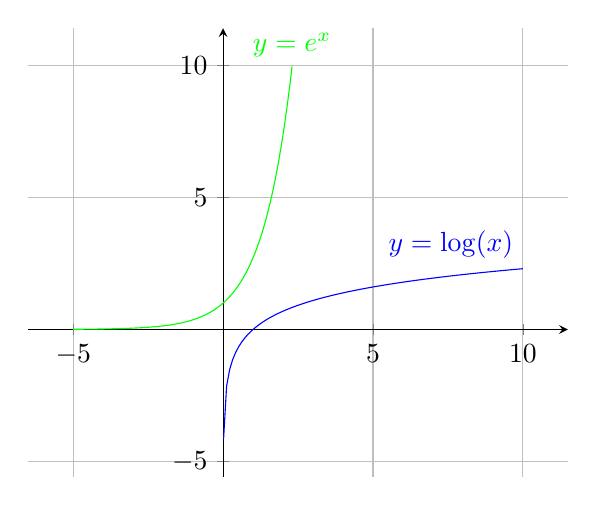
\begin{tikzpicture}
			\begin{axis}[grid=both,
			xmax=10,ymax=10,
			axis lines=middle,
			restrict y to domain=-7:12,
			enlargelimits]
			\addplot[green,domain=-5:2.3,samples=100]  {pow(e,x)} node[above]{$y=e^x$};
			\addplot[blue,domain=1/2^6:10,samples=100]  {ln	(x)} node[above left] {$y=\log(x)$};
			\end{axis}
			\end{tikzpicture}
			\caption{Exponential and Logarithm Functions}
			\label{expLogGraph}
		\end{figure}
	\end{defn}
	\begin{prop}
		Let $x,y\in R$, then we have the following:
		\begin{itemize}
			\item $e^{x+y} = e^x e^y$
			\item $\brac{e^x}^y = e^{xy}$
			\item $e^{-x} = 1/e^x$
			\item $e^0 = 1$
			\item $\log\brac{xy} = \log\brac{x} + \log\brac{y}$
			\item $\log\brac{1/x} = -\log\brac{x}$
			\item $\log\brac{x/y} = \log\brac{x} - \log\brac{y}$
			\item $\log\brac{x^y} = y\log\brac{x}$
			\item $\log\brac{1} = 0$
		\end{itemize}
	\end{prop}
	\begin{defn}
		Suppose we have a right angled triangle, let $\theta \neq \pi/2$ be an angle in the right angled triangle, the length of the opposite side to $theta$ be $O$, the length of the hypotenuse (the longest side of the triangle) be $H$ and the length of other adjacent side be $A$. 
		\begin{figure}[H]
			\centering
			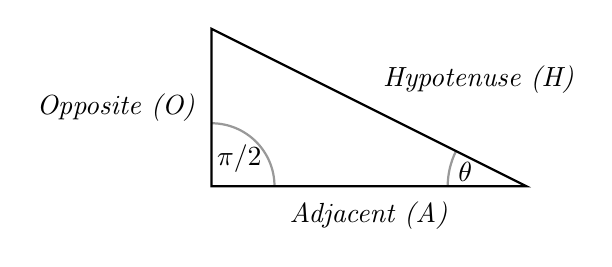
\begin{tikzpicture}[thick]
			\coordinate (O) at (0,0);
			\coordinate (A) at (4,0);
			\coordinate (B) at (0,2);
			\draw (O)--(A)--(B)--cycle;
			
			\tkzLabelSegment[below=2pt](O,A){\textit{Adjacent (A)}}
			\tkzLabelSegment[left=2pt](O,B){\textit{Opposite (O)}}
			\tkzLabelSegment[above right=2pt](A,B){\textit{Hypotenuse (H)}}
			
			\tkzMarkAngle[fill= orange,size=0.8cm,%
			opacity=.4](A,O,B)
			\tkzLabelAngle[pos = 0.5](A,O,B){$\pi/2$}
			
			\tkzMarkAngle[fill= orange,size=1.0cm,%
			opacity=.4](B,A,O)
			\tkzLabelAngle[pos = 0.8](B,A,O){$\theta$}
					
			\end{tikzpicture}
			\caption{Right Angled Triangle}
			\label{RATrigangle}	
		\end{figure}
		We define the \emph{sine} function, denoted by $\sin\brac{\cdot}$, using the following:
		$$ \sin\brac{\theta} := \frac{O}{H}$$
		We define the \emph{cosine} function similarly, denoted by $\cos\brac{\cdot}$, using the following:
		$$ \cos\brac{\theta} := \frac{A}{H}$$
		Finally, we define the \emph{tangent} function, denoted by $\tan\brac{\cdot}$, using the following:
		$$ \tan\brac{\theta} := \frac{O}{A}$$
		\begin{figure}[H]
			\centering
			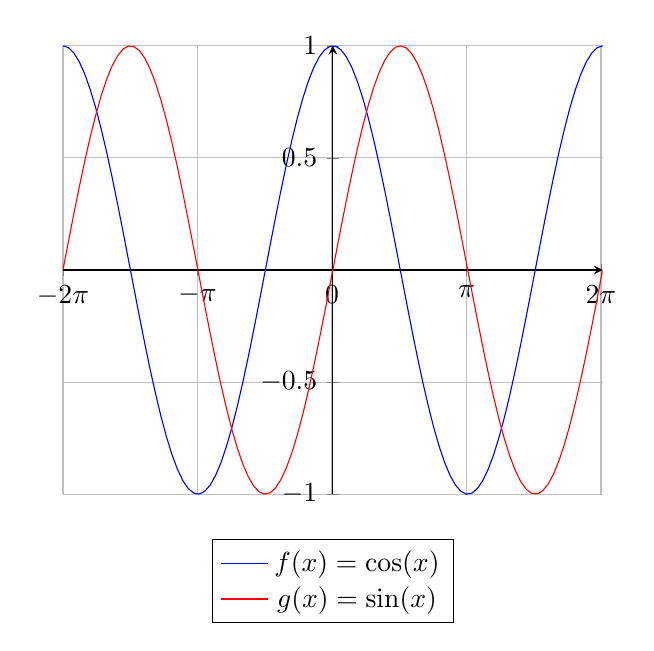
\begin{tikzpicture}
			\begin{axis}[
			enlargelimits=false,
			axis lines=middle,
			xtick={-6.28318, -3.15159265, ..., 6.28318},
			xticklabels={$-2\pi$,$-\pi$,0,$\pi$,$2\pi$},
			grid=major,
			legend style={at={(0.5,-0.1)},anchor=north}
			]
			\addplot+[no marks,domain=-2*pi:2*pi, samples=100]{cos(deg(x))};
			\addlegendentry{$f(x)=\cos(x)$}
			\addplot+[no marks,domain=-2*pi:2*pi, samples=100]{sin(deg(x))};
			\addlegendentry{$g(x)=\sin(x)$}
			\end{axis}
			\end{tikzpicture}
			\caption{Sine and Cosine Functions}
			\label{trigGraph}
		\end{figure}
	\end{defn}
	\begin{prop}
		\begin{itemize}
			\item Sine function is an odd function so $\sin\brac{-x} = -\sin\brac{x}$ and it is $2\pi$ periodic so $\sin\brac{x+2\pi} = \sin\brac{x}$ for all $x\in \R$.
			\item Cosine function is an even function so $\cos\brac{-x} = \cos\brac{x}$ and it is $2\pi$ periodic so $\cos\brac{x+2\pi} = \cos\brac{x}$ for all $x\in \R$.
			\item We have:
			$$ \tan\brac{x} = \frac{\sin\brac{x}}{\cos\brac{x}}, \quad\forall x\in \R$$
			Tangent function is an odd function so $\tan\brac{-x} = -\tan\brac{x}$ and it is $\pi$ periodic so $\tan\brac{x+\pi} = \tan\brac{x}$ for all $x\in \R$.
			\item $$\cos^2\brac{x} + \sin^2\brac{x} = 1$$
			\item $$ \sin\brac{x\pm y} = \sin\brac{x}\cos\brac{y} \pm \sin\brac{y}\cos\brac{y}$$
			\item $$ \cos\brac{x\pm y} = \cos\brac{x}\cos\brac{y}\mp \sin\brac{x}\sin\brac{y}$$
			\item $$ \tan\brac{x\pm y} = \frac{\tan\brac{x}+\tan\brac{y}}{1\mp \tan\brac{x}\tan\brac{y}}$$
			\item $$\sin\brac{x+\pi/2} = \cos\brac{x}, \quad \cos\brac{\pi/2 - x} = \sin\brac{x}$$
		\end{itemize}
	\end{prop}
	\begin{defn}
		We define reciprocals of the trigonometric functions \emph{cosecant}, \emph{secant} and \emph{cotangent} by the following:
		$$ \csc\brac{x} := \frac{1}{\sin\brac{x}}, \quad \sec\brac{x} := \frac{1}{\cos\brac{x}}, \quad \cot\brac{x} := \frac{1}{\tan\brac{x}}$$
	\end{defn}
	\begin{defn}
		We define the \emph{hyperbolic} functions as the following:
		\begin{eqnarray*}
			\sinh\brac{x} &:=& \frac{e^{x}-e^{-x}}{2}\\
			\cosh\brac{x} &:=& \frac{e^{x}+e^{-x}}{2}\\
			\tanh\brac{x} &:=& \frac{\sinh\brac{x}}{\cosh\brac{x}}
		\end{eqnarray*}
	\end{defn}
	\begin{prop}
		\begin{itemize}
			\item $$\tanh\brac{x} = \frac{e^{2x}-1}{e^{2x}+1} $$
			\item $$ \cosh^2\brac{x} - \sinh^2\brac{x} = 1$$
			\item $$ \sinh\brac{x+y} = \sinh\brac{x}\cosh\brac{y} + \sinh\brac{y}\cosh\brac{x}$$
			\item $$\cosh\brac{x+y} = \cosh\brac{x}\cosh\brac{y} + \sinh\brac{x}\sinh\brac{y}$$
		\end{itemize}
	\end{prop}
	\begin{lemma}
		The inverse function for $\sinh\brac{\cdot}$ is:
		$$ \sinh^{-1}\brac{x} = \log\brac{\abs{x+\sqrt{x ^2 +1}}}$$
	\end{lemma}
	\begin{proof}
		\begin{eqnarray*}
			y &=& \sinh^{-1}\brac{x}\\
			%&\Updownarrow&\\
			\sinh\brac{y} &=& x \\
			%&\Updownarrow &\\
			\frac{e^y-e^{-y}}{2} &=& x\\
			%&\Updownarrow &
			e^{2y} -2xe^y -1 &=& 0\\
			e^y &=& \frac{2x\pm \sqrt{4x^2+4}}{2}\\
			e^y &=& x \pm \sqrt{x^2 + 1}\\
		&&	(\text{As } \sqrt{x^2 + 1} > x \text{ and } e^y>0,  \forall y \in \R)\\
			e^y &=& x + \sqrt{x^2 + 1}\\
			y &=& \log\brac{\abs{x+\sqrt{x^2 + 1}}}
		\end{eqnarray*}
	\end{proof}
	\begin{lemma}
		\begin{itemize}
			\item $$\cosh^{-1}\brac{x} = \log\brac{\abs{x+\sqrt{x^2 -1}}}$$
			\item $$\tanh^{-1}\brac{x} = \frac{1}{2}\log\brac{\abs{\frac{1+x}{1-x}}}$$
		\end{itemize}
	\end{lemma}
	\begin{lemma}
		The following tables describes the domains and images of the previous functions we have looked at:
		\begin{table}[H]
			\centering
			\begin{tabular}{c|c|c|c}
				{\bf Function} & {\bf Domain} & {\bf Image} & {\bf Odd/Even/Neither }\\\hline
				$\exp\brac{\cdot}$ & $\R$ & $\R_{>0}$& Neither\\\hline
				$\log\brac{\cdot}$ & $\R_{>0}$ & $\R$ & Neither\\\hline
				$\sin\brac{\cdot}$ & $\R$ & $\sqbrac{-1,1}$ & Odd\\\hline
				$\cos\brac{\cdot}$ & $\R$ & $\sqbrac{-1,1}$ & Even\\\hline
				$\tan\brac{\cdot}$ & $\R\backslash\curlbrac{\brac{2n+1}\pi/2:n\in \Z}$ & $\R$ & Odd\\\hline
				$\sinh\brac{\cdot}$ & $\R$ & $\R$ & Odd\\\hline
				$\cosh\brac{\cdot}$ & $\R$ & $\left[1,\infty\right)$ & Even\\\hline
				$\tanh\brac{\cdot}$ & $\R$ & $\brac{-1,1}$ & Odd\\\hline
				$\sinh^{-1}\brac{\cdot}$ & $\left[1,\infty\right)$ & $\R_{\geq 0}$ & Odd\\\hline
				$\cosh^{-1}\brac{\cdot}$ & $\R$ & $\left[1,\infty\right)$ & Neither\\\hline
				$\tanh^{-1}\brac{\cdot}$ &$\brac{-1,1}$& $\R$ & Odd\\
			\end{tabular}
			\caption{Domains, images and other properties of key functions}
			\label{domImFunc}
		\end{table}
	\end{lemma}
\subsection{Differentiation}
	We would want to know about the rate of change of a function with elements in its domain.
	\begin{defn}
		Let $f:X\rightarrow Y$ be a function and $x_0 \in X$, we define the \emph{differential} of $f$ at $x_0$ by the following if the limit exists and is unique:
		$$ f'\brac{x_0} = \lim_{\delta\rightarrow 0}\frac{f\brac{x_0 + \delta}-f\brac{x_0}}{\delta}$$
	\end{defn}
	\begin{lemma}
		Let $f:X\rightarrow Y$ be a function and $x_0\in X$. If $f$ is differentiable at $x_0$ then $f$ is continuous at $x_0$.
	\end{lemma}
	\begin{proof}
		We want to prove the following:
		$$\lim_{x\rightarrow x_0} f\brac{x} = f\brac{x_0}$$
		We use the following which follows from being differentiable:
		\begin{eqnarray*}
			\lim_{x\rightarrow x_0} \brac{\frac{f\brac{x}-f\brac{x_0}}{x-x_0}} &=& f'\brac{x_0}\\
			&\Updownarrow&\\
			\lim_{x\rightarrow x_0} \brac{f\brac{x}-\brac{x_0}} &=& \brac{\lim_{x\rightarrow x_0} \brac{x- x_0}}f'\brac{x_0}\\
			&\Updownarrow&\\
			\lim_{x\rightarrow x_0} \brac{f\brac{x}-\brac{x_0}} &=& 0
		\end{eqnarray*}
	\end{proof}
	\begin{rmk}
		The converse is not true and we can use $f\brac{x} = \abs{x}$ as the counter example as $f$ is continuous everywhere but not differentiable at 0 as the limit is not unique:
		$$\lim_{x\rightarrow 0^+} f'\brac{x} = 1 \neq -1 = \lim_{x\rightarrow 0^-} f'\brac{x}$$
	\end{rmk}
	There are different notations, we can use:
	$$ f'\brac{x} \brac{\text{Lagrange}} = \diff{f}{x} \brac{\text{Leibniz}} = Df \brac{\text{Euler}}$$
	Where $D$ can be thought of as a differential operator which maps from a function space to a function space. We will also have $\dot{y} \brac{\text{Newton}}$ notation which will be used to for differentiation with time.
	\begin{prop}
		\begin{itemize}
			\item $$\diff{}{x}\brac{x^n} = nx^{n-1}$$
			\item $$\diff{}{x}\brac{e^x} = e^x$$
			\item $$\diff{}{x}\brac{e^{ax}} = ae^{ax}$$
			\item $$\diff{}{x}\brac{\log\brac{x}} = \frac{1}{x}$$
			\item $$\diff{}{x}\brac{\sin\brac{x}} = \cos\brac{x}$$
			\item $$\diff{}{x}\brac{\cos\brac{x}} = -\sin\brac{x}$$
			\item $$\diff{}{x}\brac{\tan\brac{x}} = \sec^2\brac{x}$$
		\end{itemize}
	\end{prop}
	\begin{defn}
		We say a map $T:X\rightarrow Y$ is linear if for all $\lambda,\mu\in \R, x_1, x_2\in X$ we have:
		$$ T\brac{\lambda x_1 + \mu x_2} = \lambda T\brac{x_1} + \mu T\brac{x_2}$$
	\end{defn}
	\begin{prop}
		Let $f,g:X\rightarrow Y$ be differentiable functions and $\lambda,\mu\in \R$. The differential operator is linear which means for all $x\in X$ we have:
		$$ D\brac{\lambda f\brac{x} + \mu g\brac{x}} = \lambda D\brac{f\brac{x}} + \mu D\brac{g\brac{x}}$$
	\end{prop}
	\begin{prop}[Product rule]
		Let $f,g:X\rightarrow Y$ be differentiable functions then for all $x\in X$ we have:
		$$ D\brac{f\brac{x}g\brac{x}} = f'\brac{x}g\brac{x} + f\brac{x}g' \brac{x}$$
	\end{prop}
	\begin{prop}[Chain Rule]
		Let $f:X\rightarrow Y, g:Y\rightarrow Z$ be differentiable functions then for all $x\in X$ we have:
		$$ D\brac{f\brac{g\brac{x}}} = g'\brac{x}\cdot f'\brac{g\brac{x}}$$
	\end{prop}
	\begin{prop}[Quotient Rule]
		Let $f,g:X\rightarrow Y$ be differentiable functions then for all $x\in X$ we have:
		$$ D\brac{\frac{f\brac{x}}{g\brac{x}}} = \frac{f'\brac{x}g\brac{x} - f\brac{x}g'\brac{x}}{\brac{g\brac{x}}^2}$$
	\end{prop}
	\begin{lemma}
		Let $a\in\R$ and $y = a^x$, then we have:
		$$ \frac{dy}{dx} = a^x\log\brac{a}$$
	\end{lemma}
	\begin{proof}
		We have to use implicit differentiation here:
		\begin{eqnarray*}
			y &=& a^x\\
			&\Updownarrow&\\
			\log\brac{y} &=& x\log\brac{a}\\
			&\Downarrow&\\
			\frac{1}{y}\cdot\diff{y}{x} &=& \log\brac{a}\\
			&\Updownarrow&\\
			\diff{y}{x} &=& y\log\brac{a}\\
			&\Updownarrow&\\
			\diff{y}{x} &=& a^x \log\brac{a}
		\end{eqnarray*}
	\end{proof}
	\begin{rmk}
		Not all functions are differentiable everywhere so we have to be careful around singularities such as $1/x$ when $x=0$ or $1/\brac{x-2}$ when $x=2$.
	\end{rmk}
	\begin{prop}[Leibniz Rule]
		Let $f,g:X\rightarrow Y$ be differentiable functions and $n\in\N$ then we have:
		$$D^n\brac{fg} = \sum_{k=0}^n \binom{n}{k}D^k\brac{f}D^{n-k}\brac{g}$$
	\end{prop}
	\begin{prop}[L'Hospital's Rule]
		Let $f,g:X\rightarrow Y$ be differentiable functions, $x_0\in X$ such that the following limit exists:
		$$\lim_{x\rightarrow x_0} \frac{f'\brac{x}}{g'\brac{x}}$$
		And we have the following:
		$$ \lim_{x\rightarrow x_0} f\brac{x} = \lim_{x\rightarrow x_0} g\brac{x} = 0 \text{ or } \pm \infty$$
		Then we have:
		$$\lim_{x\rightarrow x_0} \frac{f\brac{x}}{g\brac{x}}=\lim_{x\rightarrow x_0} \frac{f'\brac{x}}{g'\brac{x}}$$
	\end{prop}
\subsection{Taylor Series}
	We want to find local polynomial approximations to complicated functions, we use Taylor series to do this.
	\begin{defn}
		Let $f:X\rightarrow Y$ be a function and $x_0\in X$. We define its Taylor series around $x_0$ by the following:
		$$ f\brac{x} = \sum_{k=0}^{\infty} \frac{f^{\brac{k}}\brac{x_0}\brac{x-x_0}^k}{k!}$$
	\end{defn}
	We should really check for convergence but we will not worry about that here. The following proposition can be proved by finding the coefficients of the Taylor series for each function which can be done by finding the correct differentials and evaluating them at the right point.
	\begin{prop}
		\begin{itemize}
			\item $$ e^x = \sum_{k=0}^{\infty}\frac{x^k}{k!}, \quad \forall x\in \R$$
			\item $$ \log\brac{1+x} = \sum_{k=0}^{\infty} \frac{\brac{-1}^k x^{k+1}}{k+1}, \quad \forall \abs{x}<1$$
			\item $$\log\brac{1-x} = -\sum_{k=0}^{\infty}\frac{x^{k+1}}{k+1}, \quad \forall \abs{x}<1$$
			\item $$ \frac{1}{1-x} = \sum_{k=0}^{\infty} x^{k}, \quad \forall \abs{x}<1$$
			\item $$ \sin\brac{x} =\sum_{k=0}^{\infty} \frac{\brac{-1}^k x^{2k+1}}{\brac{2k+1}!}, \quad \forall x\in \R$$
			\item $$ \cos\brac{x} = \sum_{k=0}^{\infty} \frac{\brac{-1}^k x^{2k}}{\brac{2k}!}, \quad \forall x\in \R$$
			\item $$ \sinh\brac{x} =\sum_{k=0}^{\infty} \frac{ x^{2k+1}}{\brac{2k+1}!}, \quad \forall x\in \R$$
			\item $$ \cosh\brac{x} = \sum_{k=0}^{\infty} \frac{x^{2k}}{\brac{2k}!}, \quad \forall x\in \R$$
		\end{itemize}
	\end{prop}
	\begin{thm}[Binomial Theorem]
		Let $n\in\N$ and $x\in\R$ such that $\abs{x}<1$ then we have:
		$$ \brac{1+x}^n = \sum_{k=0}^{\infty} \binom{n}{k}x^{k}$$
	\end{thm}
\subsection{Integration}
	\begin{defn}
		Let $f:X\rightarrow Y$ be a function. We definite an operator called \emph{indefinite integral} which maps from a function space to another function space. We use the following notation:
		$$f\mapsto \int f\brac{x}dx$$
		We define the indefinite integral by:
		$$ F\brac{x} := \int f\brac{x}dx, \quad \text{do that}  \quad \diff{F}{x}\brac{x} = f\brac{x}$$
	\end{defn}
	\begin{rmk}
		Since the derivative of a constant $c\in\R$ is 0, the indefinite integral of any function is only determined up to an arbitrary constant.
	\end{rmk}
	\begin{prop}
		Let $a\neq 0\in\R$.
		\begin{itemize}
			\item $$\int x^n dx = \frac{x^{n+1}}{n+1} + c$$
			\item $$\int e^{ax} dx = \frac{e^{ax}}{a} + c$$
			\item $$\int \frac{1}{x} dx = \log\brac{x} + c$$
			\item $$\int \sin\brac{ax} dx = -\frac{\cos\brac{ax}}{a} + c$$
			\item $$\int \cos\brac{ax} dx = \frac{\sin\brac{ax}}{a} + c$$
		\end{itemize}
	\end{prop}
	\begin{lemma}
		The indefinite integral operator is linear. Let $f,g:X\rightarrow Y$ be functions and $\lambda,\mu\in\R$ then we have the following:
		$$ \int \brac{\lambda f\brac{x} + \mu g\brac{x}}dx = \lambda\int f\brac{x}dx + \mu\int g\brac{x}dx$$
	\end{lemma}
	\begin{defn}
		Let $f:X\rightarrow Y$ be a function and $a,b\in X$. The \emph{definite integral operator} is a map which maps functions into the reals. The definite integral takes in a function and two elements from the function's domain which are called \emph{limits} and outputs a real number. The following is the notation for the definite integral for the function $f$ between the limits $a$ and $b$:
		$$\int_{a}^{b} f\brac{x} dx$$
	\end{defn}
	\begin{rmk}
		The geometric understand behind the definite integral is the area under the function (between the function and the x-axis) between the to limits.
	\end{rmk}
	\begin{eg}
		\begin{itemize}
			\item $$\int_{1}^{3} x^3 dx = \sqbrac{\frac{x^4}{4}}_1^3 = \frac{1}{4}\brac{3^4 - 1^4} = 20$$
			\item $$\int_{-1}^{1}e^x dx = \sqbrac{e^x}_{-1}^1 = e - 1/e$$
		\end{itemize}
	\end{eg}
	\begin{lemma}
		The definite integral operator is linear, given the same limits. Let $f,g:X\rightarrow Y$ be functions, $a,b\in X$ and $\lambda,\mu\in\R$ then we have the following:
		$$\int_{a}^{b}\brac{\lambda f\brac{x} + \mu g\brac{x}}dx = \lambda\int_{a}^{b}f\brac{x}dx + \mu\int_{a}^{b}g\brac{x}dx$$
	\end{lemma}
	\begin{prop}
		Let $f:X\rightarrow Y$ be a function and $a\geq b \geq c\in X$. then we have the following:
		\begin{itemize}
			\item $$\int_{a}^{c} f\brac{x}dx = \int_{a}^{b}f\brac{x}dx + \int_{b}^{c}f\brac{x}dx$$
			\item $$\int_{a}^{b} f\brac{x}dx = - \int_{b}^{a}f\brac{x}dx$$
		\end{itemize}
	\end{prop}
	\begin{thm}[Integration by Substitution]
		Let $f:X\rightarrow Y, g:Y\rightarrow Z$ be functions,  $f$ is invertible and $y_1,y_2\in Y$. Then we have the following:
		$$ \int_{y_1}^{y_2} g\brac{y}dy = \int_{x_1 = f^{-1}\brac{y_1}}^{x_2 = f^{-1}\brac{y_2}} g\brac{f\brac{x}}f'\brac{x}dx$$
	\end{thm}
	\begin{proof}['Proof']
		We make a substitution $y= f\brac{x}$ hence we have:
		$$\diff{y}{x} = f'\brac{x} \Rightarrow dy = f'\brac{x} dx$$
		So have have:
		\begin{eqnarray*}
			\int_{y_1}^{y_2} g\brac{y} dy &=& \int_{y_1}^{y_2} g\brac{f\brac{x}} dy\\
			&=& \int_{x_1 = f^{-1}\brac{y_1}}^{x_2 = f^{-1}\brac{y_2}} g\brac{f\brac{x}}f'\brac{x}dx
		\end{eqnarray*}
	\end{proof}
	\begin{thm}[Integration by Parts]
		Let $f:X\rightarrow Y$ be a function and $a\leq b\in X$. Suppose there exist functions $u,v:X\rightarrow Y$ so that:
		$$ f\brac{x} = \diff{u}{x}\brac{x}v\brac{x},\quad \forall x\in\sqbrac{a,b}$$
		Then we have:
		$$ \int_{a}^{b} f\brac{x}dx = \int_{a}^{b} \diff{u}{x}\brac{x}v\brac{x}dx= \sqbrac{u\brac{x}v\brac{x}}_a^b -\int_{a}^{b}u\brac{x}\diff{v}{x}\brac{x}dx$$
	\end{thm}
	\begin{proof}
		We have the following:
		$$\diff{}{x}\brac{u\brac{x}v\brac{x}} = \diff{u}{x}\brac{x}v\brac{x} + u\brac{x}\diff{v}{x}\brac{x}$$
		Which is equivalent to:
		$$\diff{u}{x}\brac{x}v\brac{x}  = \diff{}{x}\brac{u\brac{x}v\brac{x}} - u\brac{x}\diff{v}{x}\brac{x}$$
		Now integrating both side we get what we need:
		$$\int_{a}^{b} \diff{u}{x}\brac{x}v\brac{x}dx= \sqbrac{u\brac{x}v\brac{x}}_a^b -\int_{a}^{b}u\brac{x}\diff{v}{x}\brac{x}dx$$
	\end{proof}
	\begin{rmk}
		Pick $v\brac{x}$ so that $v'\brac{x}$ is 'reducing' so normally this is a polynomial and you would want to pick $du/dx$ so that it is integrable easily so something like the exponential function.
	\end{rmk}
	\begin{eg}[Reduction Formula]
		Consider the following problem:
		$$ I_n = \int_{0}^{\infty} e^{-t}t^ndt $$
		We want to use the following substitution:
		\begin{eqnarray*}
			\diff{u}{t}\brac{t} = e^{-t},&&\quad v\brac{t} = t^n\\
			u\brac{t} = -e^{-t},&&\quad \diff{v}{t}\brac{t} = nt^{n-1}
		\end{eqnarray*}
		Using the integration by parts formula we get:
		\begin{eqnarray*}
			I_n &=& \int_{0}^{\infty} e^{-t}t^ndt \\
			&=& \sqbrac{-e^{-t}t^n}_0^{\infty} - \int_{0}^{\infty}-e^{-t}nt^{n-1}dt\\
			&=& 0 + n\int_{0}^{\infty} e^{-t}t^{n-1}dt\\
			&=& n I_{n-1}\\
			&\vdots &\\
			&=& n! I_0
		\end{eqnarray*}
		Where:
		$$ I_0 = \int_{0}^{\infty}e^{-t}dt = \sqbrac{-e^{-t}}_{0}^{\infty} = -\brac{0-1} = 1$$
		Therefore we have that:
		$$ I_n = n!$$
		This is similar to the \emph{Gamma} function. 
	\end{eg}
	\begin{prop}
		Let $f:X\rightarrow Y$ be a function. We have the following result:
		$$\int \frac{f'\brac{x}}{f\brac{x}}dx = \log\brac{\abs{f\brac{x}}} + c$$
	\end{prop}
	\begin{prop}[Simple Partial Fractions]
		Let $a_0,a_1,b_0,b_1\in\R$ such that $a_0b_1-a_1b_0 \neq 0$. We have the following:
		$$ \int\frac{1}{\brac{a_1x + a_0}\brac{b_1x + b_0}}dx = \brac{\frac{1}{a_0b_1-a_1b_0}}\log\brac{\frac{b_1 x + b_0}{a_1 x + a_0}}+c$$
	\end{prop}
	\begin{proof}
		We want to equate the following and solve for $A,B$:
		$$\frac{1}{\brac{a_1 x+ a_0}\brac{b_1 x + b_0}} = \frac{A}{a_1 x + a_0}+\frac{B}{b_1 x + b_0}$$
		We have:
		$$\frac{A}{a_1 x + a_0}+\frac{B}{b_1 x + b_0} = \frac{A\brac{b_1 x + b_0} + B\brac{a_1 x + a_0}}{\brac{a_1 x + a_0}\brac{b_1 x + b_0}}$$
		Therefore we have the following equation:
		$$ 1 = x\brac{Ab_1 + Ba_1} + \brac{Ab_0 + B a_0}$$
		So equating the coefficients of $x^1=x$ and $x^0=1$ we have the following simultaneous equations:
		\begin{eqnarray}
			Ab_1 + Ba_1 &=& 0\label{eq1}\\
			Ab_0 + Ba_0 &=& 1\label{eq2}
		\end{eqnarray}
		(\ref{eq1}) implies that $A = -a_1 B/b_1$. Substituting it into (\ref{eq2}) we get:
		\begin{eqnarray*}
			\brac{-\frac{a_1 B}{b_1}}b_0 + Ba_0 &=& 1\\
			&\Updownarrow&\\
			B\brac{-\frac{a_1b_0}{b_1} + a_0} &=& 1\\
			&\Updownarrow&\\
			B &=& \frac{b_1}{a_0b_1 - a_1b_0}
		\end{eqnarray*}
		Now solving for $A$ we get:
		$$ A = -\frac{a_1}{a_0b_1-a_1b_0}$$
		Now we integrate:
		\begin{eqnarray*}
			\int \frac{1}{\brac{a_1 x+ a_0}\brac{b_1 x + b_0}}dx &=& A\int\frac{1}{a_1 x + a_0}dx+B\int\frac{1}{b_1 x + b_0}dx\\
			&=& \brac{-\frac{a_1}{a_0b_1-a_1b_0}}\int\frac{1}{a_1 x + a_0}dx + \brac{\frac{b_1}{a_0b_1 - a_1b_0}}\int\frac{1}{b_1 x + b_0}dx\\
			&=& \brac{-\frac{a_1}{a_0b_1-a_1b_0}}\frac{1}{a_1}\log\brac{a_1x + a_0} + \brac{\frac{b_1}{a_0b_1 - a_1b_0}}\frac{1}{b_1}\log\brac{b_1 x + b_0} + c\\
			&=&\brac{\frac{1}{a_0b_1-a_1b_0}}\brac{\log\brac{b_1 x + b_0} - \log\brac{a_1x + a_0}}+c\\
			&=&\brac{\frac{1}{a_0b_1-a_1b_0}}\log\brac{\frac{b_1 x + b_0}{a_1 x + a_0}}+c
		\end{eqnarray*} 
	\end{proof}
\subsection{Complex Numbers}
	\begin{defn}
		We define a complex number $z\in\C$ where $z=x+iy$ for $x,y\in \R$ and $i = \sqrt{-1}$. It follows that $i^2 = -1$.\\ \\
	\end{defn}
	\begin{defn}
		Let $z = x+iy, z_1 = x_1+iy_1, z_2 = x_2+iy_2\in\C$ for some $x,y,x_1,y_1,x_2,y_2\in\R$.
		\begin{itemize}
			\item We define the \emph{complex conjugate} of $z$ by:
			$$\overline{z} := x-iy$$
			\item We define the \emph{norm} of $z$ by:
			$$\abs{z} := \sqrt{x^2+y^2} = \sqrt{z\cdot\overline{z}}$$
			\item We 'define' the following operations:
				$$z_1 \pm z_2 = \brac{x_1 \pm x_2} + i\brac{y_1\pm y_2}$$
				$$z_1\times z_2 = \brac{x_1 + iy_1}\brac{x_2+iy_2}
				= x_1x_2 +iy_1x_2 + ix_1y_2 +i^2 y_1y_2 = \brac{x_1x_2 - y_1y_2} + i\brac{x_1y_2 + x_2y_1}$$
				$$\frac{z_1}{z_2} =\frac{x_1+iy_1}{x_2+iy_2}= \frac{x_1+iy_1}{x_2+iy_2}\times\frac{x_2-iy_2}{x_2-iy_2} = \frac{\brac{x_1x_2+y_1y_2}+i\brac{-x_1y_2 + x_2y_1}}{x_2^2+y_2^2}$$
		\end{itemize}
	\end{defn}
	\begin{prop}
		Let $z,z_1,z_2\in\C$.
		\begin{itemize}
			\item $\overline{\brac{\overline{z}}} = z$
			\item $\overline{z_1 + z_2} = \overline{z_1} + \overline{z_2}$
			\item $\overline{\brac{z_1\cdot z_2}} = \overline{z_1}\cdot \overline{z_2}$
			\item $\brac{z+\overline{z}}/2 = \repart{z}=:\text{Real part of } z$
			\item $\brac{z-\overline{z}}/2 = \impart{z}=:\text{Imaginary part of } z$
			\item $\brac{z\cdot\overline{z}} = \abs{z}^2$
			\item $\abs{\overline{z}}^2 = \overline{z}\cdot\overline{\brac{\overline{z}}} = \overline{z}\cdot z = \abs{z}^2$
			\item $\frac{z_1}{z_2} = \frac{z_1}{z_2}\times\frac{\overline{z_2}}{\overline{z_2}} = \frac{z_1z_2}{\abs{z_2}^2}$
			\item $\abs{z_1z_2}^2 = \abs{z_1}^2\abs{z_2}^2$
		\end{itemize}
	\end{prop}
	\begin{thm}[Euler's Formula]
		Let $\theta\in\R$, then we have:
		$$e^{i\theta} = \cos\brac{\theta}+i\sin\brac{\theta}$$
	\end{thm}
	\begin{prop}
		For any $z =x + iy \in\C$ for some $x,y\in\R$, we can also write it in the modulus argument form:
		$$ z = re^{i\theta} = r\brac{\cos\brac{\theta}+i\sin\brac{\theta}}$$
		Where:
		$$ r = \sqrt{x^2+y^2} = \abs{z},\quad \theta = \arctan\brac{\frac{y}{x}}$$
	\end{prop}
	\begin{prop}
		Let $z_1=r_1e^{i\theta_1},z_2 = r_2e^{i\theta_2}\in\C$ where $r_1,r_2,\theta_1,\theta_2\in\R$. Then we have:
		\begin{itemize}
			\item $$z_1z_2 = r_1r_2e^{i\brac{\theta_1+\theta_2}}$$
			\item Suppose $r_2 \neq 0$, then:
			$$\frac{z_1}{z_2}=\frac{r_1}{r_2}e^{i\brac{\theta_1-\theta_2}}$$
		\end{itemize}
	\end{prop}
\subsection{Multi-Variate Calculus}
	\begin{defn}
		Let $f:X\times Y\rightarrow Z$ be a multivariate function. We define the \emph{partial derivative} of $f$ with respect to $x\in X$ as:
		$$\pardiff{f}{x} := \lim_{\delta\rightarrow 0}\frac{f\brac{x+\delta,y}-f\brac{x,y}}{\delta} = f_x$$
		Similarly the partial derivative of $f$ with respect to $y\in Y$ is defined as:
		$$\pardiff{f}{x} := \lim_{\delta\rightarrow 0}\frac{f\brac{x,y+\delta}-f\brac{x,y}}{\delta} = f_y$$
		We also define \emph{higher order} derivatives of $f$ as following:
		$$\pardiff{^2 f}{x^2} = \pardiff{}{x}\brac{\pardiff{f}{x}},\quad  \pardiff{^2 f}{y^2} = \pardiff{}{y}\brac{\pardiff{f}{y}},\quad \pardiff{^2 f}{xy} = \pardiff{}{x}\brac{\pardiff{f}{y}},\quad \pardiff{^2 f}{yx} = \pardiff{}{y}\brac{\pardiff{f}{x}}$$
	\end{defn}
	\begin{thm}
		Let $f:X\times Y\rightarrow Z$ be a function. Suppose the second order derivatives exist and are continuous then we have:
		$$ f_{xy} = \pardiff{^2f}{xy} =\pardiff{^2 f}{yx} = f_{yx}$$
	\end{thm}
	\begin{lemma}
		Let $f:X\times Y \rightarrow Z$ be a function. Suppose $f\brac{x,y} = f\brac{x\brac{t},y\brac{t}}$. Then we have:
		$$\diff{f}{t}\brac{t} = \pardiff{f}{x}\brac{x\brac{t},y\brac{t}}\diff{x}{t}\brac{t} + \pardiff{f}{y}\brac{x\brac{t},y\brac{t}}\diff{y}{t}\brac{t}$$
	\end{lemma}
	\begin{lemma}
		Let $f:X\times Y \rightarrow Z$ be a function. Suppose $f\brac{x,y} = f\brac{x\brac{u,v},y\brac{u,v}}$. Then we have:
		$$\pardiff{f}{u} = \pardiff{f}{x}\pardiff{x}{u} + \pardiff{f}{y}\pardiff{y}{u}$$
		$$\pardiff{f}{v} = \pardiff{f}{x}\pardiff{x}{v} + \pardiff{f}{y}\pardiff{y}{v}$$
	\end{lemma}
	\begin{thm}
		Let $f:X\times T\rightarrow Y$ be a function and $x_0\in X, t_0\in T$ then we have the multivariate Taylor series as:
		\begin{eqnarray*}
		f\brac{x,t} =&& f\brac{x_0,t_0} + \brac{x-x_0}f_x\brac{x_0,t_0}+ \brac{t-t_0}f_t\brac{x_0,t_0} + \dots\\ &&\dots+\frac{1}{2}\brac{ \brac{x-x_0}^2f_{xx}\brac{x_0,t_0}+2\brac{x-x_0}\brac{t-t_0}f_{xt}\brac{x_0,t_0}+\brac{t-t_0}^2f_{tt}\brac{x_0,t_0}}
		\end{eqnarray*}
	\end{thm}
	\begin{eg}
		We have:
		$$f\brac{x+\delta_x,y+\delta_y} = f\brac{x,y} + \delta_x f_x\brac{x,y} + \delta_yf_y\brac{x,y} +\frac{f_{xx}\brac{x,y}\delta_x^2}{2} + f_{xy}\delta_x\delta_y +\frac{f_{yy}\brac{x,y}\delta_y^2}{2} + O\brac{\delta_x^2,\delta_y^2}$$
		We use the following notation:
		$$df:=\lim_{\delta_x\rightarrow 0,\delta_y\rightarrow 0}\brac{f\brac{x+\delta_x,y+\delta_y} -f\brac{x,y}}$$
		So we have the first order approximation:
		$$df \approx \delta_x\pardiff{f}{x}+\delta_y\pardiff{x}{y}$$
	\end{eg}
\subsection{Probability Problems}
\subsubsection{Birthday Problem}
	Suppose we have a room with $n\in\N$ people. We want to know the probability of at least two people in the room sharing birthdays. We need to make a few assumptions to start with:
	\begin{enumerate}
		\item There are 365 days in a year.
		\item The event of a person's birth is independent of anyone else's birth.
		\item The probability of a person's birthday on a given day is uniformly distributed.
	\end{enumerate}
	Now that we have made these assumptions, let us define the event $X$ to be the random variable which denotes the number of pairs of people that share birthdays:
	\begin{eqnarray*}
	\prob{\curlbrac{X\geq 1}} &=& 1- \prob{\curlbrac{X\geq 1}^c}\\
	&=&1-\prob{\curlbrac{X<1}}\\
	&=&1-\prob{\curlbrac{X = 0}}
	\end{eqnarray*}
	So we now have to find $\prob{\curlbrac{X=0}}$ which is the probability of the event where no pair of people share a birthday. To find the probability of no two people sharing the same birthday, we can do this iteratively, let us define the event:
	$$A_n = \curlbrac{\text{No two people share a birthday in a room of $n$ people}}$$
	$A_1$ is the same is saying the one person in the room can have their birthday on any day of the year. 
	\begin{eqnarray*}
		\prob{A_1} &=& \prob{\bigcup_{d_1 = 1}^{365}\curlbrac{B_1 = d_1}}\\
		&=& \sum_{d_1=1}^{365}\prob{\curlbrac{B_1 = d_1}}\\
		&=& \sum_{d_1=1}^{365}\frac{1}{365}\\
		&=&\frac{365}{365}\\
		&=&1
	\end{eqnarray*}
	Where $\curlbrac{B_i = d_i}$ is the event that the $i$-th person's birthday happens on $d_i$-th day of the year. Now let us try $n=2$, let us define the event $A_2 = \curlbrac{\text{No two people share a birthday in a room with two people}}$:
	\begin{eqnarray*}
		\prob{A_2} &=& \prob{\bigcup_{d_1=1}^{365}\bigcup_{\substack{d_2=1\\ d_2\neq d_1}}^{365}\brac{\curlbrac{B_1 = d_1}\cap\curlbrac{B_2=d_2}}}\\
		&=& \brac{\sum_{j=1}^{365}\prob{\curlbrac{B_1 = d_j}}}\times\brac{\sum_{k=2}^{365}\prob{\curlbrac{B_2 = d_k}}|\curlbrac{B_1 = d_j}}
	\end{eqnarray*}
	
\section{Transition Probability}

\subsection{Forward Kolmogorov Equation}
	\begin{prop}[Forward Kolmogorov Equation Derivation]
		Let $x\in\R$ and $s>0$, consider a trinomial random walk which starts at point $x$ at time $s$. Let $\alpha < 1/2$, the probability of an up move of $\dy$ is $\alpha$, down move of $-\dy$ is $\alpha$ and remaining in the same position is $1-2\alpha$ over a time period of $\dt$. Let $y\in\R$ and $t>0$, defining $p\brac{y,t;x,s}$ to be the probability of moving from $\brac{x,s}$ to $\brac{y,t}$, $p$ satisfies the following partial differential equation:
		\begin{equation}\label{forwardKolmogorovEqn}
			\pardiff{p}{t} = c^2 \pardiff{^2p}{y^2}
		\end{equation}
	\end{prop}
	\begin{proof}
		To find the probability of going from $\brac{x,s}$ to $\brac{y,t}$, we would like to go a timestep back to $t-\dt$ and look at the relationship from there. At timestep $t-\dt$ we could have been at $y+\dy$, $y$ or $y-\dy$. Therefore leaving the dependency on $\brac{x,s}$, we have the following equation:
		$$p\brac{y,t} = \alpha p \brac{y-\dy,t-\dt} + \alpha p\brac{y+\dy,t-\dt} + \brac{1-2\alpha}p\brac{y,t-\dt}$$
		
		Therefore, we can expand all the terms on the right using Taylor expansion for the first order terms for $t$ and second order terms for $y$:
		
		\begin{eqnarray*}
			p\brac{y,t} &=& \alpha \brac{p\brac{y,t}-\dt\pardiff{p}{t} - \dy\pardiff{p}{y} + \frac{1}{2}\dy^2\pardiff{^2p}{y^2}} + \dots\\
			&\cdots+ & \alpha \brac{p\brac{y,t}-\dt\pardiff{p}{t} + \dy\pardiff{p}{y} + \frac{1}{2}\dy^2\pardiff{^2p}{y^2}} + \dots\\
			&\cdots+ & \brac{1-2\alpha} \brac{p\brac{y,t}-\dt\pardiff{p}{t}}
		\end{eqnarray*}
		
		Cancelling out terms, we get the following:
		
		\begin{eqnarray*}
			0 &=& \alpha\dy^2\pardiff{^2p}{y^2} - \dt\pardiff{p}{t}\\
			&\Updownarrow&\\
			\pardiff{p}{t}&=& \alpha \frac{\dy^2}{\dt} \pardiff{^2p}{y^2}
		\end{eqnarray*}
		
		Assuming that $\dy^2$ is proportional to $\dt$ and letting $c^2 = \alpha \dy^2/\dt$, we get the following partial differential equation:
		
		$$\pardiff{p}{t}= c^2 \pardiff{^2p}{y^2}$$	
		
	\end{proof}
	
	\begin{prop}\label{forwardKolmogorovSolnProp}
		Let $x,y\in\R$ and $s,t>0$, suppose we want the transition probability of going from $\brac{x,s}$ to $\brac{y,t}$, denoted by $p\brac{y,t;x,s}$, and we know that it satisfies the \hyperref[forwardKolmogorovEqn]{Forward Kolmogorov Equation}:
		$$\pardiff{p}{t}= c^2 \pardiff{^2p}{y^2}$$
		Then we have the following result:
		\begin{equation}\label{forwardKolmogorovSoln}
			p\brac{y,t;x,s} = \frac{1}{2c\sqrt{\pi\brac{t-s}}}\exp\brac{\frac{\brac{y-x}^2}{4c^2\brac{t-s}}}
		\end{equation}
	\end{prop}
	\begin{proof}
		Suppose $p\brac{y,t}$ satisfies the \hyperref[forwardKolmogorovEqn]{Forward Kolmogorov Equation}, then we use the method of similarity to obtain a solution. Suppose the solution is of the following form:
		$$p\brac{y,t} = t^\alpha f\brac{\frac{y}{t^\beta}} = t^\alpha f\brac{\xi},\quad \xi = \frac{y}{t^\beta} $$
		Then we have the following differentials:
		\begin{eqnarray*}
			\pardiff{p}{t} &=& \alpha t^{\alpha -1}f\brac{\xi} + t^\alpha f'\brac{\xi}\pardiff{\xi}{t}\\
			&=& \alpha t^{\alpha -1}f\brac{\xi} + t^\alpha f'\brac{\xi}\brac{ -bt^{-b-1}y}\\
			&=& t^{\alpha -1}\brac{\alpha f\brac{\xi} -b\xi f'\brac{\xi}}\\
			\pardiff{p}{y} &=& t^\alpha f'\brac{\xi}\pardiff{\xi}{y} = t^{\alpha-\beta} f'\brac{\xi}\\
			\pardiff{^2p}{y^2} &=& t^{\alpha-\beta} f''\brac{\xi}\pardiff{\xi}{y} = t^{\alpha-2\beta} f''\brac{\xi}
		\end{eqnarray*}
		Therefore, we have the following relation:
		\begin{eqnarray*}
			\pardiff{p}{t} &=& c^2 \pardiff{^2p}{y^2}\\
			&\Updownarrow& \\
			t^{\alpha -1}\brac{\alpha f\brac{\xi} -b\xi f'\brac{\xi}} &=& c^2t^{\alpha-2\beta} f''\brac{\xi}
		\end{eqnarray*}
		For the above equation to have a similarity solution, both sides of the equation have to be independent of $t$ hence we need:
		$$\alpha -1 = \alpha - 2\beta \Leftrightarrow \beta = \frac{1}{2}$$
		Therefore we have:
		$$p\brac{y,t} = t^\alpha f\brac{\xi} = t^\alpha f\brac{\frac{y}{\sqrt{t}}}$$
		As $p\brac{y,t}$ is a transition probability, we must have that the integral over $y\in\R$ should add up to one:
		\begin{eqnarray*}
			\int_{y\in\R}p\brac{y,t}dy &=& 1 \\
			&\Updownarrow&\\
			t^\alpha\int_{y\in\R}f\brac{\frac{y}{\sqrt{t}}}dy &=& 1\\
			\brac{\text{Subsititute } u = y/\sqrt{t},~ du = dy/\sqrt{t}}&\Updownarrow&\\
			t^{\alpha+1/2}\int_{u\in\R}f\brac{u}du &=& 1 
		\end{eqnarray*}
		Again we need the above relation ship to be true for all $t>0$, therefore, we need:
		$$\alpha + \frac{1}{2} = 0 \Leftrightarrow \alpha = -\frac{1}{2}$$
		Now we have the following differential equation:
		\begin{eqnarray*}
			t^{\alpha -1}\brac{\alpha f\brac{\xi} -b\xi f'\brac{\xi}} &=& c^2t^{\alpha-2\beta} f''\brac{\xi}\\
			&\Updownarrow&\\
			-t^{-1/2}\frac{1}{2}\brac{f\brac{\xi} + \xi f'\brac{\xi}}&=& c^2t^{-1/2}f''\brac{\xi}\\
			&\Updownarrow&\\
			-\frac{1}{2c^2}d\brac{\xi f\brac{\xi}} &=& f''\brac{\xi}\\
			&\Updownarrow&\\
			-\frac{1}{2c^2}\xi f\brac{\xi} &=& f'\brac{\xi} + K
		\end{eqnarray*}
		For a fixed $t>0$, we have that $f\brac{\xi}\rightarrow 0$ and $f'\brac{\xi}\rightarrow 0$ as $\xi\rightarrow\infty$ due to the fact that its part of a probability density function. This will mean that $K=0$. Therefore, we now have the following differential equation:
		\begin{eqnarray*}
			-\frac{1}{2c^2}\xi f\brac{\xi} &=& f'\brac{\xi}\\
			&\Updownarrow& \\
			\frac{f'\brac{\xi}}{f\brac{\xi}} &=& -\frac{1}{2c^2}\xi\\
			&\Updownarrow& \\
			f\brac{\xi} &=& A\exp\brac{-\frac{1}{4c^2}\xi^2}
		\end{eqnarray*}
		Where $A$ is a normalising constant which calculated the following way:
		\begin{eqnarray*}
			A\int_{\xi\in\R}\exp\brac{-\frac{1}{4c^2}\xi^2} &=& 1\\
			\brac{\text{Subsititute } u = \xi/\brac{2c},~ du = d\xi/\brac{2c}}&\Updownarrow&\\
			2cA\underbrace{\int_{u\in\R}\exp\brac{-u^2} }_{=\sqrt{\pi}}&=& 1\\
			&\Updownarrow&\\
			A &=& \frac{1}{2c\sqrt{\pi}}			
		\end{eqnarray*}
		Therefore we have the fundamental solution:
		\begin{eqnarray*}
			p\brac{y,t} &=& t^{-1/2}f\brac{\xi}\\
			&=& \frac{1}{2c\sqrt{\pi t}}f\brac{\frac{y}{\sqrt{t}}}\\
			&=& \frac{1}{2c\sqrt{\pi t}}\exp\brac{-\frac{1}{4c^2t}y^2}
		\end{eqnarray*}
		As you can see this is the Gaussian probability density function with $\mu = 0$ and $\sigma = c\sqrt{2t}$.\\
		
		We need that $p\brac{x,s} = p\brac{x,s;x,s} = 1$. To achieve this we need to adjust our fundamental solution to get the right answer. We need to have a Gaussian probability density function with $\mu = x$ and $\sigma = t-s$ as we should have that $\sigma\downarrow 0 $ as $t\downarrow s$. Therefore, we have the following final solutions:
		
		$$p\brac{y,t;x,s} = \frac{1}{2c\sqrt{\pi\brac{t-s}}}\exp\brac{-\frac{\brac{y-x}^2}{4c^2\brac{t-s}}}$$
		
	\end{proof}
	
\section{$ \sigma_t \propto \sigma_1 \sqrt{t} $}
	
	We have that the volatility of the returns of an asset scales with square root of time. Assume $X_m$ denotes the discrete asset price at period $m$. Then we define the $n$-period return from $X_m$ to $X_{m+n}$, $r_{m+n,n}$, as: 
	$$ X_{n+m} = X_m \exp\brac{r_{m+n,n}} \Leftrightarrow r_{m+n,n} = \log\brac{\frac{X_{n+m}}{X_m}} $$
	Suppose we know the distribution of $r_{i,1}:=r_i$ which is i.i.d. with variance $\sigma^2$. Then we know that $\V{\log\brac{\frac{X_{m+1}}{X_m}}} = \V{r_{m+1}} = \sigma^2$ which means that the volatility which is the standard deviation of the returns for one period is $\sigma$. From here, we can show that the $n$-period volatility scales with $\sqrt{n}$ by the following:
	\begin{eqnarray*}
		\V{\log\brac{\frac{X_{m+n}}{X_m}}} &=& \V{\sum_{i=m+1}^{m+n}r_i}\\
		&=& \sum_{i=m+1}^{m+n}\sum_{j=m+1}^{m+n}\text{cov}\brac{r_i,r_j}\\
		&=& \sum_{i=m+1}^{m+n}\V{r_i} + 2\sum_{i=m+1}^{m+n}\sum_{j>i}^{m+n}\underbrace{\text{cov}\brac{r_i,r_j}}_{= 0 \text{ as returns are i.i.d.}}\\
		&=& n \sigma^2
	\end{eqnarray*}
\section{Stochastic Calculus}

	\begin{thm}[Ito's Lemma]\label{itosLemma}
		Let $\brac{X_t^i:t>0}$ be stochastic processes for $i=1,\dots,n$ where $n\in\N$. Let $f_t = f(t,X^1_t,\dots,X^n_t)$ be a function of time and the stochastic processes. Then we have the following:
		\begin{equation}\label{intIto}
		f_t = f_s +  \int_{s}^{t}\pardiff{f_r}{r}dr + \sum_{i=1}^{n}\int_{s}^{t}\pardiff{f_r}{X^i_r}dX^i_r + \frac{1}{2}\sum_{i=1}^{n}\sum_{j=1}^{n}\int_{s}^{t}\pardiff{^2f_r}{X_r^iX_r^j}d\pbrac{X^i,X^j}_r
		\end{equation}
		Which is equivalent to the following:
		\begin{equation}\label{ito}
			df_t = \pardiff{f_t}{t}dt + \sum_{i=1}^{n}\pardiff{f_t}{X^i_t}dX^i_t + \frac{1}{2}\sum_{i=1}^{n}\sum_{j=1}^{n}\pardiff{^2f_t}{X_t^iX_t^j}d\pbrac{X^i,X^j}_t
		\end{equation}
		Where $\pbrac{X^i,X^j}_t$ is the quadratic variation process of $X^i$ and $X^j$.
	\end{thm}
	
	\begin{cor}
		Let $\brac{B_t^i:t>0}$ for Brownian motions for $i=1,\dots,n$ where $n\in\N$. Let $f_t = f(t,B^1_t,\dots,B^n_t)$ be a function of time and the stochastic processes. Let the quadratic variation process between $B^i_t$ and $B^j_t$ for $i,j=1,\dots,n$ be $\pbrac{B^i,B^j}_t = \rho_{i,j}dt$. Then we have the following:
		\begin{equation}\label{bmIto}
			df_t = \brac{\pardiff{f_t}{t} +\frac{1}{2}\sum_{i=1}^{n}\pardiff{^2f_t}{B^i_t} + \rho_{i,j}\sum_{i=1}^{n}\sum_{j>i}^{n}\pardiff{^2f_t}{B^i_tB^i_j} }dt + \sum_{i=1}^{n}\pardiff{f_t}{B^i_t}dB^i_t 
		\end{equation}
	\end{cor}
\subsection{Geometric Brownian Motion}
	\begin{prop}
		Let $X_t$ follow a geometric Brownian motion such that: 
		\begin{equation}\label{gbm}
			dX_t = \mu X_t dt + \sigma X_t dB_t
		\end{equation}
		Where $\mu,\sigma\in\R$. Then we have the following formula for $X_t$ where $s<t$:
		\begin{equation}\label{gbmSol}
			X_t = X_s\exp\brac{\brac{\mu - \frac{1}{2}\sigma^2}\brac{t-s} + \sigma\brac{B_t - B_s}}
		\end{equation}
	\end{prop}
	\begin{proof}
		Let us look at the function $\log\brac{X_t}$. We can use \hyperref[itosLemma]{Ito's Lemma} to get the following:
		\begin{eqnarray*}
			d\brac{\log\brac{X_t}} &=& \pardiff{\log\brac{X_t}}{X_t}dX_t + \frac{1}{2}\pardiff{^2\log\brac{X_t}}{X_t^2}d\pbrac{X,X}_t\\
			&=& \frac{1}{X_t}\brac{\mu X_t dt + \sigma X_t dB_t} + \frac{1}{2}\brac{-\frac{1}{X_t^2}}\sigma^2 X_t^2 d\pbrac{B,B}_t\\
			&=& \mu dt + \sigma dB_t -\frac{1}{2}\sigma^2 dt\\
			&=& \brac{\mu - \frac{1}{2}\sigma^2}dt + \sigma dB_t
		\end{eqnarray*}
		Now integrating both sides between times $s$ and $t$, we get the following:
		\begin{eqnarray*}
			\int_{s}^{t}d\brac{\log\brac{X_t}} &=& \brac{\mu-\frac{1}{2}\sigma^2}\int_{s}^{t}dr + \sigma\int_{s}^{t}dB_r\\
			&\Updownarrow&\\
			\log\brac{X_t} - \log\brac{X_s} &=& \brac{\mu-\frac{1}{2}\sigma^2}\brac{t-s} + \sigma\brac{B_t - B_s}\\
			&\Updownarrow&\\
			X_t &=& X_s\exp\brac{\brac{\mu-\frac{1}{2}\sigma^2}\brac{t-s} + \sigma\brac{B_t - B_s}}
		\end{eqnarray*}
	\end{proof}
\subsection{Vasicek Model}
	\begin{prop}
		Let $X_t$ satisfy the following stochastic differential equation:
		\begin{equation}\label{vasicek}
			dX_t = \gamma\brac{\theta - X_t}dt + \sigma dB_t
		\end{equation}
		Where $\gamma,\theta,\sigma\in\R$ and $B_t$ is a Brownian motion. Then we have the following formula for $X_t$ where $s<t$:
		\begin{equation}\label{vasicekSol}
			X_t = X_se^{-\gamma\brac{t-s}} + \theta\brac{1-e^{-\gamma\brac{t-s}}} + \sigma\int_{s}^{t}e^{-\gamma\brac{t-r}}dB_r
		\end{equation}
	\end{prop}
	\begin{proof}
		Let $X_t$ satisfy the following stochastic differential equation shown in Equation~\ref{vasicek} then we have the following:
		\begin{eqnarray*}
			dX_t &=& \gamma\brac{\theta - X_t}dt + \sigma dB_t\\
			&\Updownarrow&\\
			dX_t + \gamma X_t dt &=& \gamma\theta dt + \sigma dB_t\\
			&\Updownarrow&\\
			d\brac{X_t e^{\gamma t}} &=& \gamma\theta e^{\gamma t} dt + \sigma e^{\gamma t} dB_t\\
			&\Updownarrow& \\
			X_t e^{\gamma t} - X_s e^{\gamma s} &=& \theta\int_{s}^{t}\gamma e^{\gamma r}dr + \sigma\int_{s}^{t}e^{\gamma r}dB_r\\
			&\Updownarrow&\\
			X_t &=& X_se^{-\gamma\brac{t-s}} + \theta\brac{1-e^{-\gamma\brac{t-s}}} + \sigma\int_{s}^{t}e^{-\gamma\brac{t-r}}dB_r			
		\end{eqnarray*}
	\end{proof}
\section{Black-Scholes Equation}
	\begin{thm}[Black-Scholes Equation]\label{BSEDeriv}
		Assumptions:
		\begin{itemize}
			\item The underlying asset follows a geometric Brownian motion as follows:
			$$ dS_t = \mu S_t dt + \sigma S_t dB_t$$
			Where $\mu,\sigma\in\R$ are constants and $B_t$ is a Brownian motion.
			\item Riskless borrowing and lending rate is constant for any tenor.
			\item Buying and selling of underlying asset and borrowing and lending of any amount is possible even fractional amounts.
			\item Possible to short the underlying asset.
			\item No taxes and transaction costs.
			\item There is no arbitrage opportunities.
		\end{itemize}
		Let $V_t = V\brac{t,S_t}$ be a derivative whose value depends on the underlying $S_t$ and time. Then we have the following partial differential equation known as the Black-Scholes Equation:
		\begin{equation}\label{BSE}
			\pardiff{V_t}{t} + \frac{1}{2}\sigma^2S^2_t\pardiff{^2V_t}{S_t^2} + rS_t\pardiff{V_t}{S_t} - rV_t = 0
		\end{equation}
	\end{thm}
	\begin{proof}
		We would like to create a hedging portfolio $\Pi_t$ such that:
		$$\Pi_t = V_t + \Delta S_t$$
		Where $\Delta$ is constant over a small time increment, it is chosen at the start of the time increment then held constant then changed at the end of the time increment. Hence we have the following differential equation:
		$$d\Pi_t = dV_t + \Delta dS_t$$
		Using \hyperref[itosLemma]{Ito's Lemma} on $V_t = V\brac{t,S_t}$, we get the following:
		\begin{eqnarray*}
			d\Pi_t &=& \pardiff{V_t}{t}dt + \frac{1}{2}\pardiff{^2V_t}{S_t^2}d\pbrac{S,S}_t + \pardiff{V_t}{S_t}dS_t - \Delta dS_t\\
			&=& \pardiff{V_t}{t}dt + \frac{1}{2}\pardiff{^2V_t}{S_t^2}\sigma^2S_t^2d\pbrac{B,B}_t + \brac{\pardiff{V_t}{S_t} - \Delta} dS_t\\
			&=& \brac{\pardiff{V_t}{t} + \frac{1}{2}\sigma^2S_t^2\pardiff{^2V_t}{S_t^2}}dt+ \brac{\pardiff{V_t}{S_t} - \Delta} dS_t
		\end{eqnarray*}
		Choosing $\Delta = \pardiff{V_t}{S_t}$, we can get rid of the $dS_t$ term. Therefore no randomness is left. This means our portfolio should grow at the riskfree rate, hence $d\Pi_t = r\Pi dt$:
		\begin{eqnarray}
			d\Pi_t &=& \brac{\pardiff{V_t}{t} + \frac{1}{2}\sigma^2S_t^2\pardiff{^2V_t}{S_t^2}}dt+ \brac{\pardiff{V_t}{S_t} - \pardiff{V_t}{S_t}} dS_t\\
			&=& \brac{\pardiff{V_t}{t} + \frac{1}{2}\sigma^2S_t^2\pardiff{^2V_t}{S_t^2}}dt\label{equalBSE1}\\
			&=& r\Pi dt\\
			&=& r\brac{V_t - \pardiff{V_t}{S_t}S_t}dt\label{equalBSE2}		
		\end{eqnarray}
		Equating Equations~\ref{equalBSE1} and \ref{equalBSE2}, we get the Black-Scholes Equation:
		\begin{eqnarray}
			\pardiff{V_t}{t} + \frac{1}{2}\sigma^2S_t^2\pardiff{^2V_t}{S_t^2} &=& r\brac{V_t - \pardiff{V_t}{S_t}S_t}\\
			&\Updownarrow&\\
			\pardiff{V_t}{t} + \frac{1}{2}\sigma^2S_t^2\pardiff{^2V_t}{S_t^2} + rS_t\pardiff{V_t}{S_t} -rV_t &=& 0
		\end{eqnarray}
	\end{proof}
	
	\begin{prop}
		We can transform the \hyperref[BSE]{Black-Scholes Equation}:
		$$ \pardiff{V}{t} + \frac{1}{2}\sigma^2S^2\pardiff{^2V}{S^2} + rS\pardiff{V}{S} -rV = 0$$
		Into the following:
		$$ \pardiff{U}{\tau} = \frac{1}{2}\sigma^2\pardiff{^2U}{x^2} $$
		Where:
		$$ V(t,S) = e^{-r\brac{T-t}}U(t,S)= e^{-r\tau}U\brac{T-\tau,e^{x-\brac{r-\sigma^2/2}\tau}}$$
	\end{prop}
	\begin{proof}
		Our first transformation is $V = Ue^{-r\brac{T-t}}$, therefore we have the following differentials:
		$$\pardiff{V}{t} = e^{-r\brac{T-t}}\brac{\pardiff{U}{t} + rU},\quad \pardiff{V}{S} = e^{-r\brac{T-t}}\pardiff{U}{S},\quad \pardiff{^2V}{S^2} = e^{-r\brac{T-t}}\pardiff{^2U}{S^2}$$
		Hence we get the following equation:
		$$  e^{-r\brac{T-t}}\brac{\pardiff{U}{t}+rU + \frac{1}{2}\sigma^2S^2\pardiff{^2U}{S^2} + rS\pardiff{U}{S} - rU} = 0$$
		As $e^{-r\brac{T-t}} > 0$, we can divide both sides by it and the $rU$ cancels giving us the following:
		$$ \pardiff{U}{t}+ \frac{1}{2}\sigma^2S^2\pardiff{^2U}{S^2} + rS\pardiff{U}{S} = 0$$
		Now we substitute $\tau' = T - t$, giving us the following differential:
		$$\pardiff{}{t} = \pardiff{}{\tau'}\cdot\pardiff{\tau'}{t} = -\pardiff{}{\tau}$$
		Therefore now we have the following equation:
		$$ \pardiff{U}{\tau'} = \frac{1}{2}\sigma^2S^2\pardiff{^2U}{S^2} + rS\pardiff{U}{S} $$
		We will now make the following substitution:
		$$\xi = \log\brac{S}$$
		So, we have the following differentials:
		$$\pardiff{}{S} = \pardiff{}{\xi}\cdot\pardiff{\xi}{S} = \frac{1}{S}\pardiff{}{\xi}$$
		\begin{eqnarray}
			\pardiff{^2}{S^2} &=& \pardiff{}{S}\brac{\frac{1}{S}\pardiff{}{\xi}} \\
			&=& -\frac{1}{S^2}\pardiff{}{\xi} + \frac{1}{S}\pardiff{}{S}\brac{\pardiff{}{\xi}}\\
			&=& -\frac{1}{S^2}\pardiff{}{\xi} +\frac{1}{S}\pardiff{\xi}{S}\pardiff{}{\xi}\brac{\pardiff{}{\xi}}\\
			&=& -\frac{1}{S^2}\pardiff{}{\xi} +\frac{1}{S^2}\pardiff{^2}{\xi^2}\\
			&=& \frac{1}{S^2}\brac{\pardiff{^2}{\xi^2}-\pardiff{}{\xi}}
		\end{eqnarray}
		Therefore we have the following differential equation:
		\begin{eqnarray*}
			\pardiff{U}{\tau'} &=& \frac{1}{2}\sigma^2S^2\pardiff{^2U}{S^2} + rS\pardiff{U}{S} \\
			&=& \frac{1}{2}\sigma^2S^2\frac{1}{S^2}\brac{\pardiff{^2U}{\xi^2}-\pardiff{U}{\xi}} + r S\frac{1}{S}\pardiff{U}{\xi}\\
			&=&\frac{1}{2}\sigma^2 \pardiff{^2U}{\xi} + \brac{r-\frac{1}{2}\sigma^2}\pardiff{U}{\xi}
		\end{eqnarray*}
		Now we make two final substitutions:
		\begin{eqnarray*}
			\tau &=& \tau'\\
			x &=& \xi + \brac{r-\frac{1}{2}\sigma^2}\tau'
		\end{eqnarray*}
		We get the following differentials:
		\begin{eqnarray*}
			\pardiff{}{\tau'} &=& \pardiff{}{\tau}\pardiff{\tau}{\tau'} + \pardiff{}{x}\pardiff{x}{\tau'} = \pardiff{}{\tau} + \brac{r - \frac{1}{2}\sigma^2}\pardiff{}{x}\\
			\pardiff{}{\xi} &=& \pardiff{}{\tau}\underbrace{\pardiff{\tau}{\xi}}_{=0} + \pardiff{}{x}\pardiff{x}{\xi}  = \pardiff{}{x}\\
			\pardiff{^2}{\xi^2} &=& \underbrace{\pardiff{}{\xi}}_{\partial /\partial x}\brac{\pardiff{}{x}} = \pardiff{^2}{x^2}
		\end{eqnarray*}
		Therefore, we get the final differential equation:
		\begin{eqnarray*}
			\pardiff{U}{\tau'} &=& \frac{1}{2}\sigma^2 \pardiff{^2U}{\xi} + \brac{r-\frac{1}{2}\sigma^2}\pardiff{U}{\xi}\\
			&\Updownarrow&\\
			\pardiff{U}{\tau} + \brac{r - \frac{1}{2}\sigma^2}\pardiff{U}{x} &=& \frac{1}{2}\sigma^2\pardiff{^2U}{x^2} +  \brac{r - \frac{1}{2}\sigma^2}\pardiff{U}{x}\\
			&\Updownarrow&\\
			\pardiff{U}{\tau} &=& \frac{1}{2}\sigma^2\pardiff{^2U}{x^2}
		\end{eqnarray*}
		Where we have:
		\begin{eqnarray*}
			V(t,S) &=& e^{-r\brac{T-t}}U(t,S)\\
			&=& e^{-r\tau'}U\brac{T-\tau',S}\\
			&=& e^{-r\tau'}U\brac{T-\tau',e^{\xi}}\\
			&=& e^{-r\tau}U\brac{T-\tau,e^{x-\brac{r-\sigma^2/2}\tau}}
		\end{eqnarray*}
	\end{proof}
	
\section{Greeks}
	We will start with the closed form formulas for vanilla European calls and puts. We use the following notation:
	\begin{itemize}
		\item $t$ - current time
		\item $T$ - time at expiry
		\item $r$ - interest rates, assumed to be constant
		\item $\sigma$ - volatility, assumed to be constant
		\item $K$ - strike price
		\item $S_t$ - price of the underlying at time $t$
		\item $C_t$ - price of the call option at time $t$
		\item $P_t$ - price of the put option at time $t$
		\item $\normcdf{z}$ is the standard normal distribution where:
		$$\normcdf{z} = \frac{1}{\sqrt{2\pi}}\int_{-\infty}^{z}e^{-x^2/2}dx$$
	\end{itemize}
	We have the following formulas for calls and puts assuming the Black-Scholes-Merton model assumptions:
	$$C_t = S_t\normcdf{d_1} - Ke^{-r\brac{T-t}}\normcdf{d_2}$$
	$$P_t = Ke^{-r\brac{T-t}}\normcdf{-d_2} - S_t\normcdf{-d_1}$$
	Where: 
	$$ d_1 = \frac{\log\brac{S_t/K}+\brac{r+\sigma^2/2}\brac{T-t}}{\sigma\sqrt{T-t}}$$
	$$d_2 = d_1 -\sigma\sqrt{T-t} = \frac{\log\brac{S_t/K}+\brac{r-\sigma^2/2}\brac{T-t}}{\sigma\sqrt{T-t}}$$
	Note that we will drop the subscripts when taking derivatives. 
	\begin{prop}\label{trick1}
		We have the following relationship:
		$$ S_t \normpdf{d_1} = Ke^{-r\brac{T-t}}\normpdf{d_2}$$
		Where:
		$$ \normpdf{z} = \pardiff{\normcdf{z}}{z} = \frac{e^{-z^2/2}}{\sqrt{2\pi}}$$
	\end{prop}
	\begin{proof}
		\begin{eqnarray*}
			\normpdf{d_1} &=& \frac{e^{-d_1^2/2}}{\sqrt{2\pi}}\\
			&=& \frac{\exp\brac{-\frac{\brac{d_2 + \sigma\sqrt{T-t}}^2}{2}}}{\sqrt{2\pi}}\\
			&=& \frac{e^{-d_2^2/2}}{\sqrt{2\pi}}\exp\brac{-d_2\sigma\sqrt{T-t}-\frac{\sigma^2\brac{T-t}}{2}}\\
			&=& \normpdf{d_2}\exp\brac{-\log\brac{S_t/K} -\brac{r-\frac{\sigma^2}{2}}\brac{T-t}-\frac{\sigma^2\brac{T-t}}{2}}\\
			&=& \normpdf{d_2}\frac{K}{S_t}e^{-r\brac{T-t}}
		\end{eqnarray*}
	\end{proof}
	\begin{prop}\label{callputparity}
		The following is the call-put parity:
		$$ S_t + P_t = C_t + Ke^{-r\brac{T-t}}$$
	\end{prop}
	\begin{proof}
		Prove using the absence of arbitrage argument.
	\end{proof}
	\begin{prop}
		$$\Delta_{C} := \pardiff{C_t}{S_t} = \normcdf{d_1}$$
		$$\Delta_{P} := \pardiff{P_t}{S_t} = \normcdf{-d_1}$$
	\end{prop}
	\begin{proof}
		Starting from the pricing formula of the call option $ C_t = S_t\normcdf{d_1} - Ke^{-r\brac{T-t}}\normcdf{d_2}$ and taking the derivative with respect to $S_t$, we get the following:
		\begin{eqnarray*}
			\Delta_C &=& \pardiff{C_t}{S_t}\\
			&=& \normcdf{d_1} + S_t\pardiff{\normcdf{d_1}}{S_t} - Ke^{-r\brac{T-t}}\pardiff{\normcdf{d_2}}{S_t}\\
			&=& \normcdf{d_1} + S_t\normpdf{d_1}\pardiff{d_1}{S_t} - Ke^{-r\brac{T-t}}\underbrace{\pardiff{d_2}{S_t}}_{=\partial d_1/\partial S_t}\\
			&=& \normcdf{d_1} + \underbrace{\brac{S_t\normpdf{d_1}-Ke^{-r\brac{T-t}}\normpdf{d_2}}}_{= 0 \text{ by Proposition \ref{trick1}}}\pardiff{d_1}{S_t}\\
			&=& \normcdf{d_1}
		\end{eqnarray*}
		Now using the call-put parity $S_t + P_t = C_t + Ke^{-r\brac{T-t}}$ and taking the derivative with respect to $S_t$ we get:
		$$ 1 + \pardiff{P_t}{S_t} = 1 + \Delta_P = \Delta_C$$
		Therefore:
		$$ \Delta_P = 1 - \Delta_C = 1 - \normcdf{d_1} = \normcdf{-d_1}$$
	\end{proof}
	\begin{prop}
		$$ \rho_C := \pardiff{C_t}{r} = Ke^{-r\brac{T-t}}\brac{T-t}\normcdf{d_2}$$
		$$ \rho_P := -\pardiff{C_t}{r} = Ke^{-r\brac{T-t}}\brac{T-t}\normcdf{-d_2}$$
	\end{prop}
	\begin{proof}
		Starting with the pricing formula for a cal option and taking the derivative with respect to $r$ we get:
		\begin{eqnarray*}
			\rho_C &=& \pardiff{C_t}{r}\\
			&=& S_t\normpdf{d_1}\pardiff{d_1}{r} - Ke^{-r\brac{T-t}}\normpdf{d_2}\underbrace{\pardiff{d_2}{r}}_{=\partial d_1/\partial r} + \brac{T-t}Ke^{-r\brac{T-t}}\normcdf{d_2}\\
			&=& \underbrace{\brac{S_t\normpdf{d_1}-Ke^{-r\brac{T-t}}\normpdf{d_2}}}_{= 0 \text{ by Proposition \ref{trick1}}}\pardiff{d_1}{r} + \brac{T-t}Ke^{-r\brac{T-t}}\normcdf{d_2}\\
			&=& \brac{T-t}Ke^{-r\brac{T-t}}\normcdf{d_2}
		\end{eqnarray*}
		Now to use the call-put parity $S_t + P_t = C_t + Ke^{-r\brac{T-t}}$ and take the derivative with respect to $r$:
		\begin{eqnarray*}
			\rho_P &=& \rho_C - \brac{T-t}Ke^{-r\brac{T-t}}\\
			&=& \brac{T-t}Ke^{-r\brac{T-t}}\brac{\normcdf{d_2}-1}\\
			&=& -\brac{T-t}Ke^{-r\brac{T-t}}\normcdf{-d_2}
		\end{eqnarray*}
	\end{proof}
	\begin{prop}
		$$\vega = \vega_C = \pardiff{C_t}{\sigma} = \vega_P = \pardiff{P_t}{\sigma} = Ke^{-r\brac{T-t}}\normpdf{d_2}\sqrt{T-t}$$
	\end{prop}
	\begin{proof}
		First let us note that $\pardiff{C_t}{\sigma} = \pardiff{P_t}{\sigma}$ by using the call-put parity. $S_t + P_t = C_t + Ke^{-r\brac{T-t}}$ and taking the derivative with respect to $\sigma$ to get:
		$$\pardiff{P_t}{\sigma} = \pardiff{C_t}{\sigma}$$
		Now let us start with the option pricing formula for a call option and take the derivative with respect to $\sigma$:
		\begin{eqnarray*}
			\vega &=& \vega_C\\
			&=& \pardiff{C_t}{\sigma}\\
			&=& S_t\normpdf{d_1}\pardiff{d_1}{\sigma} - Ke^{-r\brac{T-t}}\normpdf{d_2}\pardiff{d_2}{\sigma}\\
			&=& S_t\normpdf{d_1}\pardiff{d_1}{\sigma} - Ke^{-r\brac{T-t}}\normpdf{d_2}\brac{\pardiff{d_1}{\sigma} - \sqrt{T-t}}\\
			&=& \underbrace{\brac{S_t\normpdf{d_1}-Ke^{-r\brac{T-t}}\normpdf{d_2}}}_{= 0 \text{ by Proposition \ref{trick1}}}\pardiff{d_1}{\sigma} + Ke^{-r\brac{T-t}}\normpdf{d_2}\sqrt{T-t}\\
			&=&Ke^{-r\brac{T-t}}\normpdf{d_2}\sqrt{T-t}
		\end{eqnarray*}
	\end{proof}

\section{Bond Pricing Equation}
	
	\begin{prop}[Bond Pricing Equation Derivation]\label{BPEDeriv}
		Let $Z_t = Z\brac{t,r_t;T}$ be a security whose value depends on current time $t$, time to maturity $T$ and the spot interest rate $r_t$ which satisfies the following stochastic differential equation:
		$$dr_t = u\brac{t,r_t}dt + w\brac{t,r_t}dB_t$$
		Where $u\brac{t,r_t}$ and $w\brac{t,r_t}$ are functions and $B_t$ is a Brownian motion. Then there exists a function $\lambda\brac{t,r_t}$ such that $Z_t$ satisfies the following partial differential equation known as the Bond Pricing Equation:
		\begin{equation}\label{BPE}
			\pardiff{Z_t}{t} + \frac{1}{2}w^2\brac{t,r_t}\pardiff{^2Z_t}{r_t^2} + \brac{u\brac{t,r_t} + \lambda\brac{t,r_t}w\brac{t,r_t}}\pardiff{Z_t}{r_t} - rZ_t = 0
		\end{equation} 
	\end{prop}
	\begin{proof}
		Let $\Zone = Z^1\brac{t,r_t;T_1}$ and $\Ztwo = Z^2\brac{t,r_t;T_2}$ be two different securities. We will create a hedging portfolio $\Pi_t$ as we did in Theorem~\ref{BSEDeriv}:
		$$\Pi_t = \Zone - \Delta \Ztwo$$
		Where $\delta$ does not change over a small time increment, it is decided before the time increment then chosen again at the end of the time increment, therefore using \hyperref[itosLemma]{Ito's Lemma} we have the following:
		\begin{eqnarray*}
			d\Pi_t &=& d\Zone - \Delta d\Ztwo\\
			&=& \brac{\pardiff{\Zone}{t}+\frac{1}{2}w^2\brac{t,r_t}\pardiff{^2\Zone}{r_t^2} + u\brac{t,r_t}\pardiff{\Zone}{r_t}}dt + \cdots\\
			&\cdots& -\Delta \brac{\pardiff{\Ztwo}{t}+\frac{1}{2}w^2\brac{t,r_t}\pardiff{^2\Ztwo}{r_t^2} + u\brac{t,r_t}\pardiff{\Ztwo}{r_t}}dt + \cdots\\
			&\cdots& + \brac{\pardiff{\Zone}{r_t}-\Delta\pardiff{\Ztwo}{r_t}}dB_t
		\end{eqnarray*}
		Therefore, we can cancel out the $dB_t$ term by choosing:
		$$\Delta = \frac{\partial\Zone/\partial r_t}{\partial\Ztwo\partial r_t}$$
		Now as $\Pi_t$ is not dependent on any random terms, it has to grow with the time value of money:
		$$d\Pi_t = r\Pi_t dt = r\brac{\Zone - \frac{\partial\Zone/\partial r_t}{\partial\Ztwo\partial r_t} \Ztwo}dt$$
		Therefore, we have the following relationship:
		\begin{eqnarray*}
			d\Pi_t &=& d\Zone - \Delta d\Ztwo\\
			&=& \brac{\pardiff{\Zone}{t}+\frac{1}{2}w^2\brac{t,r_t}\pardiff{^2\Zone}{r_t^2} + u\brac{t,r_t}\pardiff{\Zone}{r_t}}dt + \cdots\\
			&\cdots& -\Delta \brac{\pardiff{\Ztwo}{t}+\frac{1}{2}w^2\brac{t,r_t}\pardiff{^2\Ztwo}{r_t^2} + u\brac{t,r_t}\pardiff{\Ztwo}{r_t}}dt\\
			&=& r\brac{\Zone - \frac{\partial\Zone/\partial r_t}{\partial\Ztwo\partial r_t} \Ztwo}dt
		\end{eqnarray*}
		Equating the $dt$ terms from the above relation and rearranging the terms we get the following:
		 \begin{equation}\label{eqn3}
		 \frac{\pardiff{\Zone}{t}+\frac{1}{2}w^2\brac{t,r_t}\pardiff{^2\Zone}{r_t^2} + u\brac{t,r_t}\pardiff{\Zone}{r_t} - r\Zone}{\pardiff{\Zone}{r_t}} = \frac{\pardiff{\Ztwo}{t}+\frac{1}{2}w^2\brac{t,r_t}\pardiff{^2\Ztwo}{r_t^2} + u\brac{t,r_t}\pardiff{\Ztwo}{r_t} - r\Ztwo}{\pardiff{\Ztwo}{r_t}}
		 \end{equation} 
		Each side of Equation~\ref{eqn3} are dependent on different $T_i$ for $i=1,2$. This means that exists a function $\alpha\brac{t,r_t}$ independent of $T_i$ for $i=1,2$ such that each side of Equation~\ref{eqn3} is equal to that. We can also drop the distinction of $i=1,2$ for $Z^i_t$ as both sides of the equation are of the same form and generalise to a security $Z_t = Z\brac{t,r_t;T}$ and we get:
		$$ \frac{\pardiff{Z_t}{t}+\frac{1}{2}w^2\brac{t,r_t}\pardiff{^2Z_t}{r_t^2} + u\brac{t,r_t}\pardiff{Z_t}{r_t} - rZ_t}{\pardiff{Z_t}{r_t}} = \alpha\brac{t,r_t}  $$
		Without loss of generality, for some function $\lambda\brac{t,r_t}$ we set:
		$$\alpha\brac{t,r_t} = \lambda\brac{t,r_t}w\brac{t,r_t}$$
		Finally rearranging, to get the Bond Pricing Equation:
		$$ \pardiff{Z_t}{t}+\frac{1}{2}w^2\brac{t,r_t}\pardiff{^2Z_t}{r_t^2} + \brac{u\brac{t,r_t} - \lambda\brac{t,r_t}w\brac{t,r_t}}\pardiff{Z_t}{r_t} - rZ_t = 0 $$
	\end{proof}
	
\section{Other}
	\begin{eqnarray}
	\E{N_1} &=& \E{N_1,T_1=T} + \E{N_1,T_1=H}\\
	&=& \E{N_1|T_1=T}\prob{T_1=T} + \E{N_1|T_1=H}\prob{T_1=H}
	\end{eqnarray}
	
	\begin{eqnarray}
	\E{N_1|T_1=T} &=& \sum_{n=1}^{\infty}n\prob{N_1=n|T_1=T}\\ &=&\sum_{n=2}^{\infty}n\prob{N_1=n|T_1=T}\\
	&=&\sum_{k=1}^{\infty}\brac{k+1}\prob{N_1=k+1|T_1=T}\\
	&=&\sum_{k=1}^{\infty}k\prob{N_1=k+1|T_1=T}+\sum_{k=1}^{\infty}\prob{N_1=k+1|T_1=T}\\
	&=&\sum_{k=1}^{\infty}k\prob{N_1=k+1|T_1=T}+1\\
	&=&\sum_{k=1}^{\infty}k\prob{\sum_{n=1}^{\infty}\ind{T_i=T,i<n}=k+1|T_1=T}+1\\
	&=&\sum_{k=1}^{\infty}k\prob{\sum_{i=1}^{k}\ind{T_i=T} + \ind{T_{k+1}=H} =k+1|T_1=T}+1\\
	&=&\sum_{k=1}^{\infty}k\prob{\sum_{i=2}^{k}\ind{T_i=T} + \ind{T_{k+1}=H} =k}+1\\
	&=&\sum_{k=1}^{\infty}k\prob{\sum_{i=1}^{k}\ind{T_i=T} + \ind{T_{k}=H} =k}+1\\
	&=&\sum_{k=1}^{\infty}k\prob{N_1 =k}+1\\
	\end{eqnarray}
	
	\begin{eqnarray}
	\E{N_1|T_1=T} &=& \E{N_1 - 1|T_1=T} + \E{1|T_1=T}
	\end{eqnarray}
	
	\begin{eqnarray*}
		\E{N_2} &=& \E{N_2|TT}\prob{TT} + \E{N_2|HT}\prob{HT} + \E{N_2|TH}\prob{TH} +\E{N_2|HH}\prob{HH}\\
		&=& 0.25\brac{2+\E{N_2}} + 0.25\brac{2+\E{N_2}} + 0.25\brac{0.5\times 3 + 0.5\brac{3+ \E{N_2}}} + 0.25\times 2\\
		&=& 2.25 + 5/8\E{N_2} + 
	\end{eqnarray*}
	

\end{document}